\documentclass[../main/main.tex]{subfiles}
\begin{document}

\chapter{Modélisation hyperspectrale}\label{ch:modelhyperspec}

\minitoc
\vspace{2cm}
Ce chapitre est consacré l'étape de construction du cube intrinsèque de
la galaxie hôte, que nous avons introduit dans le
chapitre~\ref{ch:hypergal}.

Nous présenterons dans un premier temps le relevé Pan-STARRS, les images photométriques
qui serviront de base d'information pour notre modélisation hyperspectrale et les
étapes de pré-traitement à appliquer.

Puis nous introduirons le SED Fitter \pkg{CIGALE}, qui sera utilisé pour
obtenir une SED de la galaxie à l'échelle locale, la configuration
implémentée et son application aux images photométriques.

Enfin, nous détaillerons la construction du cube intrinsèque, étape
finale de la modélisation hyperspectrale de la galaxie.
\newpage

\section{Source photométrique}
\label{sec:photosource}

Notre cadre de recherche étant au sein de la collaboration ZTF, nous
devons prévoir le fait que nous aurons des alertes d'évènements
transitoire dans tout le ciel Nord, couverture de la caméra. Par
ailleurs, le but d'\hypergal étant une modélisation de scène d'une
observation de la SEDm, la source photométrique utilisée doit avoir a
minima la même profondeur en magnitude. Enfin, la projection se faisant
de l'espace photométrique vers l'espace des observables de la SEDm, il
serait plus judicieux d'utiliser un relevé photométrique attestant d'un
meilleur seeing, pour éviter de dégrader les données.

Le relevé Pan-STARRS1 du système Pan-STARRS — Panoramic Survey Telescope and Rapid
Response System - \citep{Kaiser2002,Kaiser2010} répond à tous ces critères. C'est d'ailleurs basé sur
la première Data Release ce relevé astronomique que la procédure de calibration photométrique
de ZTF est effectuée.

\subsection{Relevé astronomique Pan-STARRS1}
\label{ssec:ps1}

Le relevé Pan-STARRS1 \citep{ChambersPS1survey} est une installation innovante d’imagerie
astronomique à grand champ,
développé à l'Institut d'astronomie de l'Université de Hawaï. Le relevé
Pan-STARRS1 vient du nom du premier télescope du projet situé à l'Observatoire Haleakala,
Pan-STARRS Telescope \#1 ou encore PS1. L'optique de PS1 est décrit dans
\citet{Hodapp2004a, Hodapp2004b, Hodapp2004c, Morgan2008}.
Ce télescope possède un miroir
primaire de 1m80 de diamètre avec une focale de 8m, et un miroir
secondaire de 0.9m. 

La caméra montée sur le télescope PS1 est la Gigapixel Camera \#1
(GPC1) de $1.4$ gigapixel, conçue au laboratoire Lincoln
\citep{Tonry2006GPC1,Tonry2008GPC1} et offrant un champ de vue d'environ
$3.3\degree$ de diamètre. 
Le plan focal de la caméra GPC1 est divisé en 60 appareils OTA CCID58
(Orthogonal Transfer Array; \citet{Tonry1997OTA,Tonry2008GPC1}), où
chacun est composé d'un réseau de 8$\times$8 CCDs (cellules). Un unique
OTA est composé de 64 cellules de 590$\times$598 pixels de
$\SI{10}{\micro\metre}$ de côté. Une illustration du plan focal de la
caméra est présentée dans la Figure~\ref{fig:gpc1focalplan}.

\begin{figure}[h]
  \begin{minipage}[c]{0.4\textwidth}
    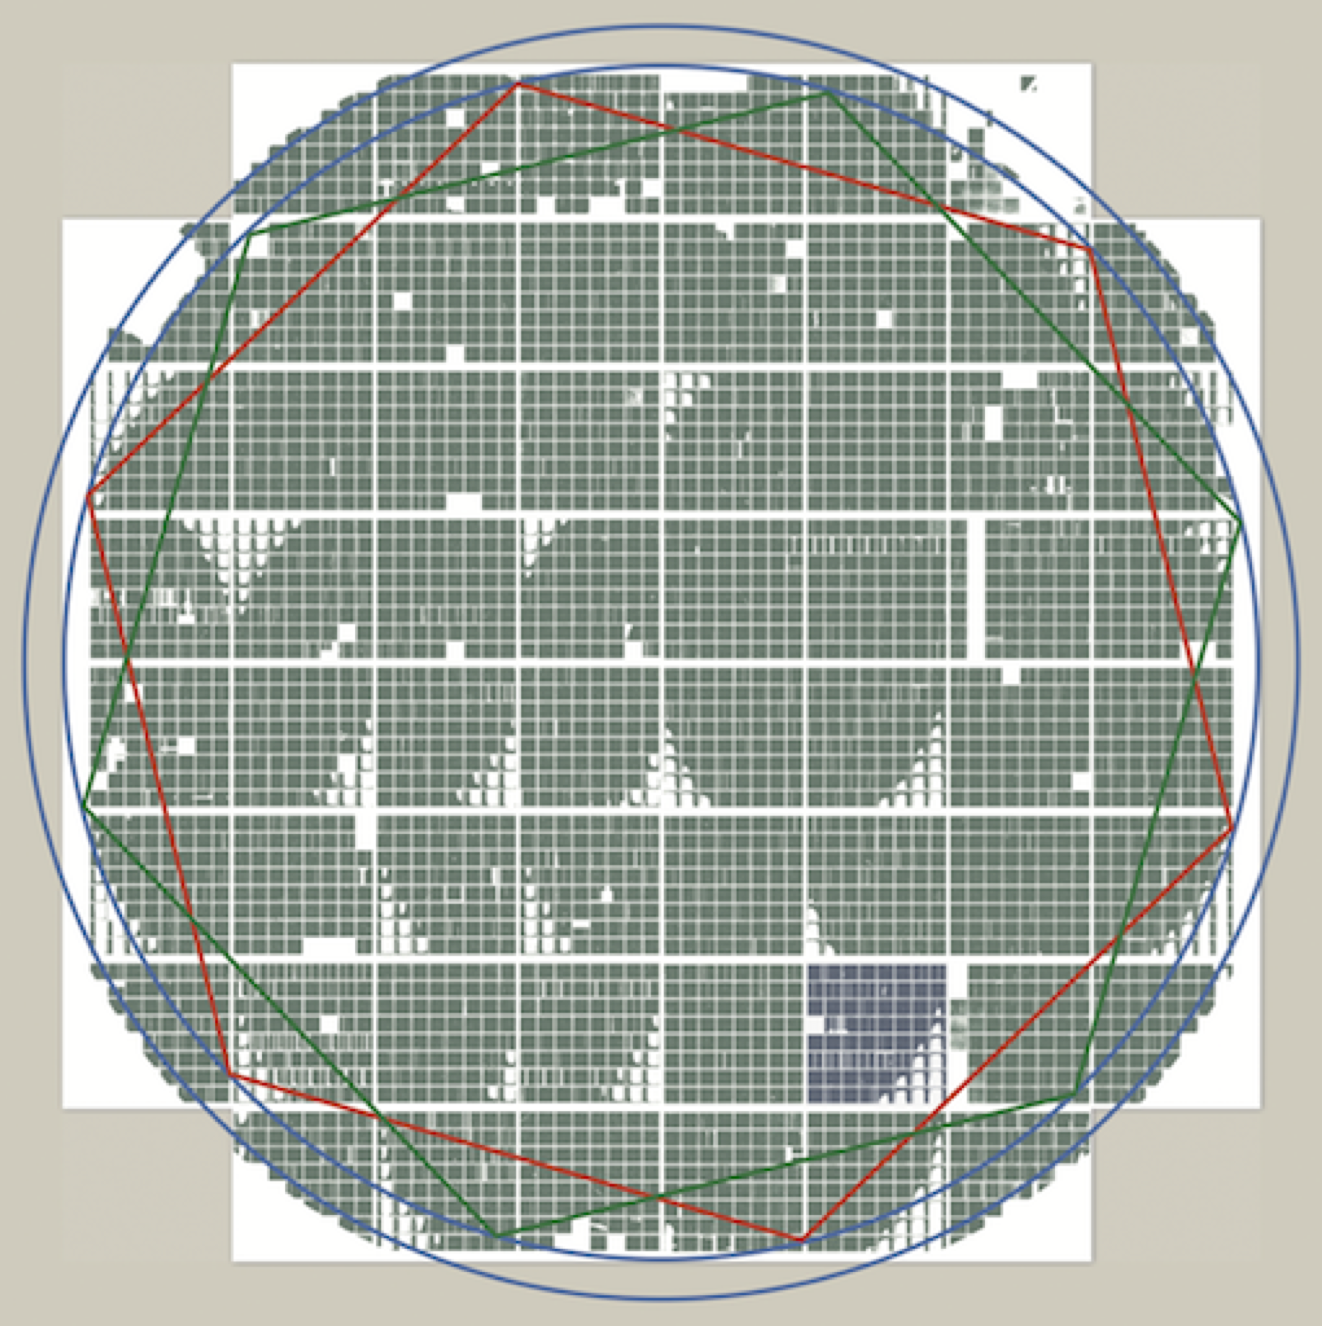
\includegraphics[width=\textwidth]{../figures/05_sedfit/GPC1focalplan.png}
  \end{minipage}\hfill
  \begin{minipage}[c]{0.5\textwidth}
    \caption[Plan focal de la Gigapixel Camera (PS1)]{Plan focal de la
    Gigapixel Camera (PS1) (figure de \citet{ChambersPS1survey}). Les cellules non fonctionnelles sont
    masquées et représentées en blanc dans la figure ci-dessus.}\label{fig:gpc1focalplan}
  \end{minipage}
\end{figure}


Une des missions de PS1 (à plus de $56\%$ du temps alloué) est l'observation de tout le ciel Nord à une déclinaison $\delta>30\degree$ :
c'est le
relevé $3\pi$ Stéradian. Les observations sont effectuées avec 5 filtres
$g_{P1}$, $r_{P1}$, $i_{P1}$, $z_{P1}$ et $y_{P1}$. On notera
l'existence d'un  sixième
filtre ($w_{P1}$) qui
englobe les filtres $g,r,i$ mais qui est utilisé pour l'étude du système
solaire et non le relevé $3\pi$ Stéradian. Les informations
de transmission de ces $6$ filtres sont présentées dans la Figure~\ref{fig:ps1filters}.

\begin{figure}
  \centering
  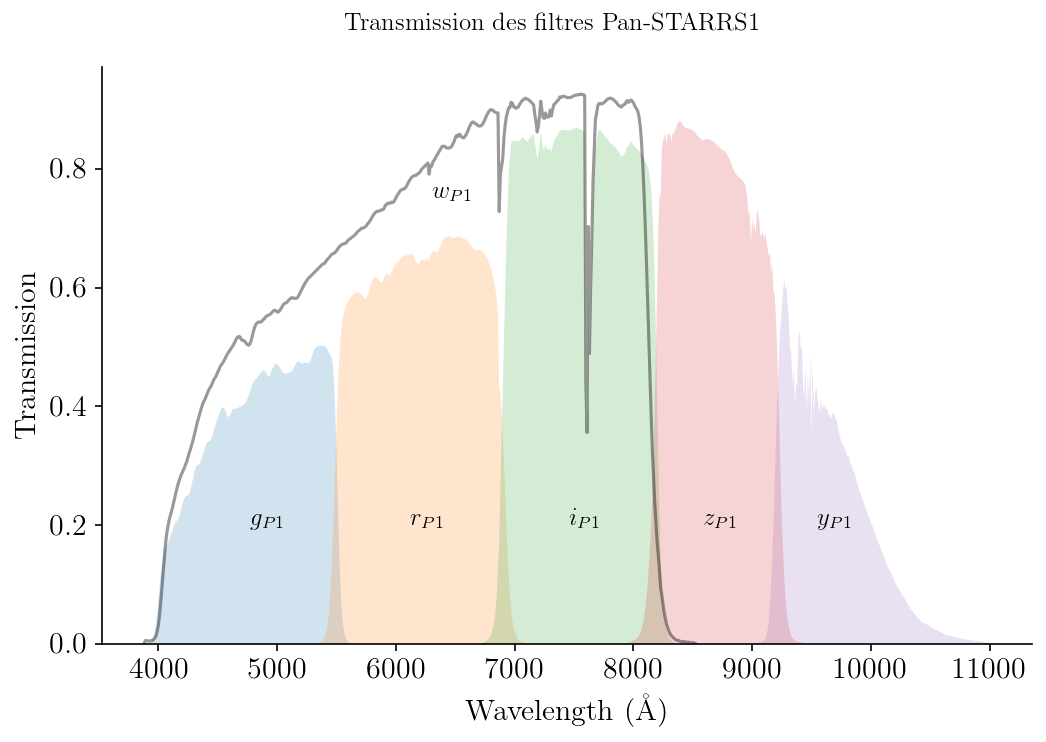
\includegraphics[width=0.8\textwidth]{../figures/05_sedfit/ps1filters.png}
  \caption[Transmission des filtres Pan-STARRS1]{Transmission des
    filtres $grizy$ de Pan-STARRS1.}
  \label{fig:ps1filters}
\end{figure}


Pan-STARRS1 utilise le système de magnitude ``AB'' \citep{Oke1983}
décrit en détail pour le relevé SDSS \citep{YorkSDSS2000} par
\citet{Fukugita1996}.

Dans ce système, une magnitude monochromatique AB est défini comme le
logarithme de la densité spectrale de flux, tel que:

\begin{align}
  \label{eq:abmag}
  m_{AB}(\nu)&= -2.5\log_{10}(f_{\nu}[\erg\ \text{s}^{-1}\cm^{-2}\Hz^{-1}]) -
  48.60\\
  m_{AB}(\nu)&\approx -2.5\log_{10}(\frac{f_{\nu}[\jy]}{3631\jy})
\end{align}

Avec $1\text{Jy} = 10^{-23}\erg.\sec^{-1}\cm^{-2}\Hz^{-1}$.

La magnitude AB d'une bande passante est alors définie telle que:
\begin{equation}
  \label{eq:abmagbp}
  m_{AB}\approx-2.5\log_{10}\left(\frac{\int
      f_{\nu}(h\nu)^{-1}A(\nu)\d\nu}{\int 3631\jy(h\nu)^{-1}A(\nu)\d\nu}   \right)
\end{equation}

Où $A(\nu)$ est la fonction de réponse du filtre considéré. Le système
photométrique de PS1 est détaillé dans \citet{Tonry2012}.

\begin{table}[h]
    \centerfloat
    \begin{threeparttable}
        \caption{Caractéristiques des filtres $grizy$ de PAN-STARRS1 et
          du relevé $3\pi$ Stéradian.}
        \label{tab:3pisteradian}
        \begin{tabular}{lccccccc}
            \toprule
             \multirow{2}[3]{*}{Filtres} & \multirow{2}[3]{*}{$\lambda_{pivot}$(\AA)} &                                                                    \multirow{2}[3]{*}{\# Expositions}  & \multirow{2}[3]{*}{\shortstack{mag
                                                  à $5\sigma$ \\(exposition unique)}} &
                                                                 \multirow{2}[3]{*}{\shortstack{mag
                                  à $5\sigma$ \\
          (expositions empilées)}} & \multirow{2}[3]{*}{\shortstack{Median
                                  \\seeing ('') }} &  \multirow{2}[3]{*}{\shortstack{Mode
                                  \\seeing ('')}} \\
          \\
            & & & & & & \\
          \midrule
          $g_{P1}$ & $4849.11$ &60528 & $22.0$ & $23.3$ & $1.47$ & $1.31$\\
          $r_{P1}$ & $6201.20$ &70918 & $21.8$ & $23.2$ & $1.31$ & $1.15$\\
          $i_{P1}$ & $7534.96$ &104414& $21.5$ & $23.1$ & $1.19$ & $1.05$\\
          $z_{P1}$ & $8674.20$ &67604 & $20.9$ & $22.3$ & $1.14$ & $1.00$\\
          $y_{P1}$ & $9627.79$ &70982 & $19.7$ & $21.4$ & $1.09$ & $0.95$\\
                     
            \bottomrule
        \end{tabular}
        \begin{tablenotes}[flushleft]
        \item \textbf{Notes.} La longueur d'onde pivot $\lambda_{pivot}$
          est déterminée avec la transmission $T(\lambda)$ tel que
          $\lambda_{pivot}=\sqrt{\frac{\int T(\lambda)\d\lambda}{\int T(\lambda)\d\lambda/\lambda^{2}}}$
        \end{tablenotes}
    \end{threeparttable}
\end{table}


Nous présentons dans la Table\ref{tab:3pisteradian} quelques
caractéristiques des filtres $grizy$ de PS1, ainsi que du relevé $3\pi$ Stéradian.
\subsection{Utilisation des images PS1}
\label{ssec:preprocessps1}


\section{\pkg{Cigale} et SEDFitting}
\label{sec:cigale}

\subsection{Présentation de Cigale}
\label{ssec:cigale}

\subsection{Utilisation}
\label{ssec:usecigale}

\section{Construction du cube intrinsèque}

\subsection{Sampling des spectres dans l'espace SEDm}
%\label{ssec:xxx}

\subsection{Construction du cube}
% \label{ssec:xxx}

%\bibliographystyle{../main/aa_url2}
%\bibliography{99_references}

\end{document}

%%% Local Variables:
%%% mode: latex
%%% TeX-master: t
%%% End:
